\begin{flushright}
    در سطح میکروپروسسورها شاهد آن بودیم که می‌توان با یک رشته از بیت‌های 0 و1، عملیات‌های مدنظر را انجام داد.
    اما صحبت با رایانه به زبان 0 و 1 بسیار سخت و دشوار بود.
    بنابراین انتزاعی بالاتر شکل گرفت تا به صورت یک مترجم دستورها را به شکل غیر از 0 و 1 دریافت کرده و به صورت رشته‌های چند بیتی به میکروپروسسور انتقال دهد.

    \begin{figure}[H]
               \centering
               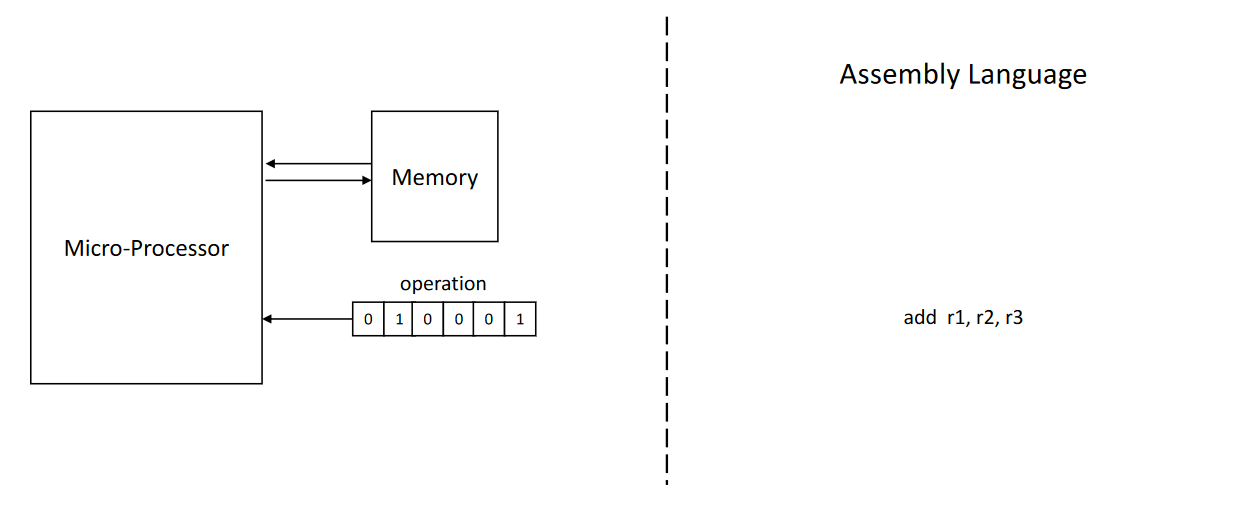
\includegraphics[scale=0.4]{source/assembly-imp&abs}
               \caption{ترجمه کد اسمبلی به رشته‌های 0 و 1}
               \label{fig:assembly-imp&abs}
    \end{figure}
\end{flushright}